\section{Bericht}

\subsection{Einleitung}
Ziel der Übung ist es mit Hilfe von Scilab bzw. Xcos eine Simulation des Balles auf einer geneigten Fläche mit Hilfe der Lösungen aus der ersten Übung aufzubauen.

\subsection{Durchführung}\begin{center}
%	\begin{minipage}{\linewidth}
%	\centering
%	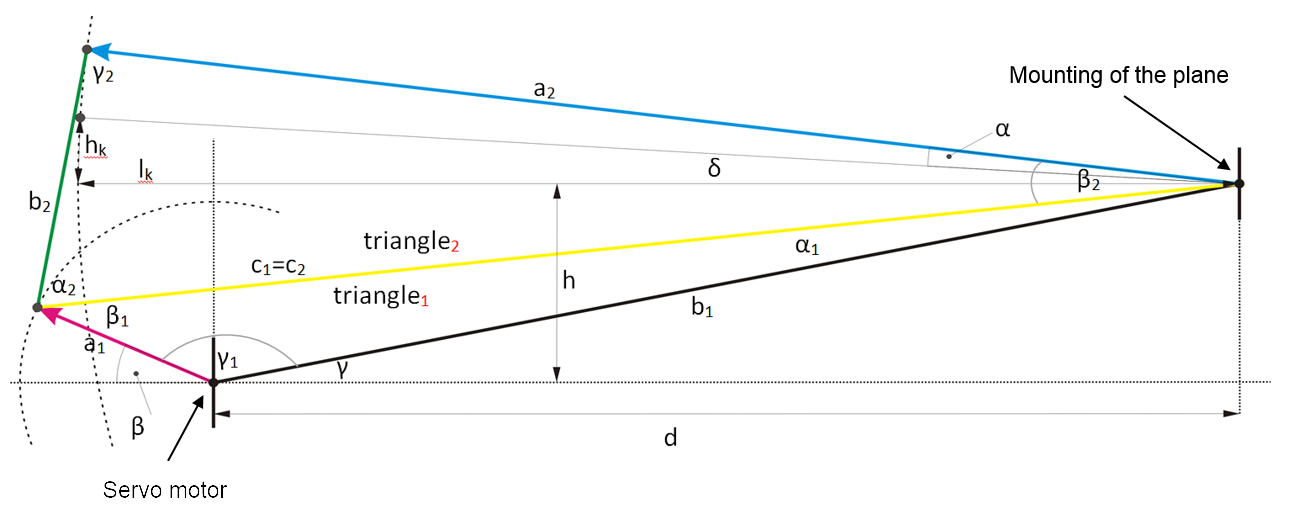
\includegraphics[scale=0.3]{images/figure1.png}
%	\captionof{figure}{Model of inclined plane}
%	\end{minipage}
\end{center}
Zuerst haben wir ein Grundgerüst der Simulation basierend auf Abbildung 1 aus der Aufgabenstellung gebaut. Im Superblock für das BOIP-Modell ...

\subsection{Besonderheiten}
text

\subsection{Fazit}
text
